\documentclass{ar2rc}

\usepackage{graphicx}
\usepackage{beraserif}
\usepackage{natbib}
\usepackage{color}


\title{An Improved Minimum-Distance Texture Estimator for Speckled Data under the $\mathcal{G}^0$ Model}
\author{Julia~Cassetti,
	Alejandro~C.~Frery}
\journal{Journal of Mathematical Imaging and Vision}
%\doi{12345}

\begin{document}
	
	\maketitle
	
	We would like to inform you that we have found an error in Figure~13 that has been fixed in this new version.
	These changes do not alter the contents of the original submission.
	
	Apart from those, we have complied with the insightful requests from the reviewer.
	
	\section{Reviewer \#1}
	
	\subsection{Summary}
	
	\fbox{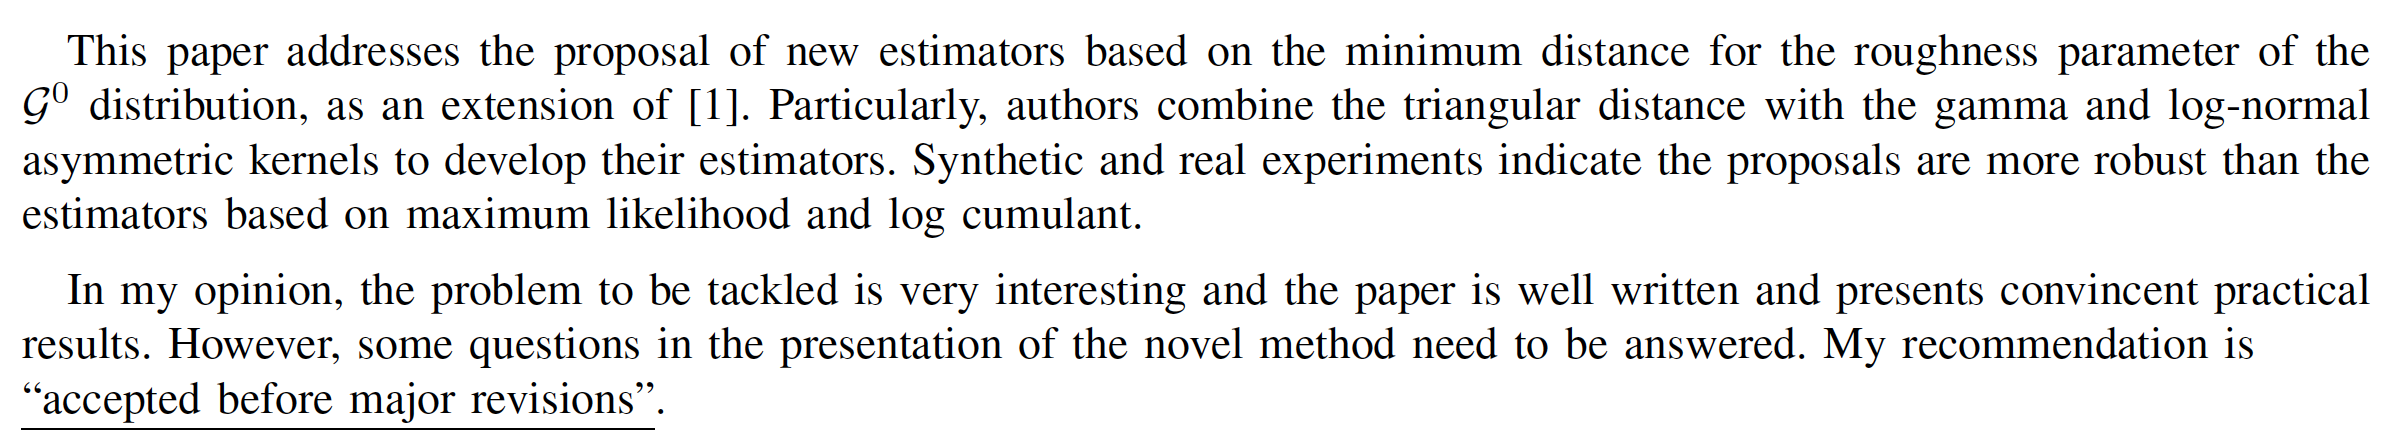
\includegraphics[width=\linewidth]{Summary}}	
	
	\AR We would like to thank the reviewer for the careful analysis of our work.
	We agree with the suggestions, and we have proceeded accordingly.
	
	\subsection{Critical comments}
	
	\fbox{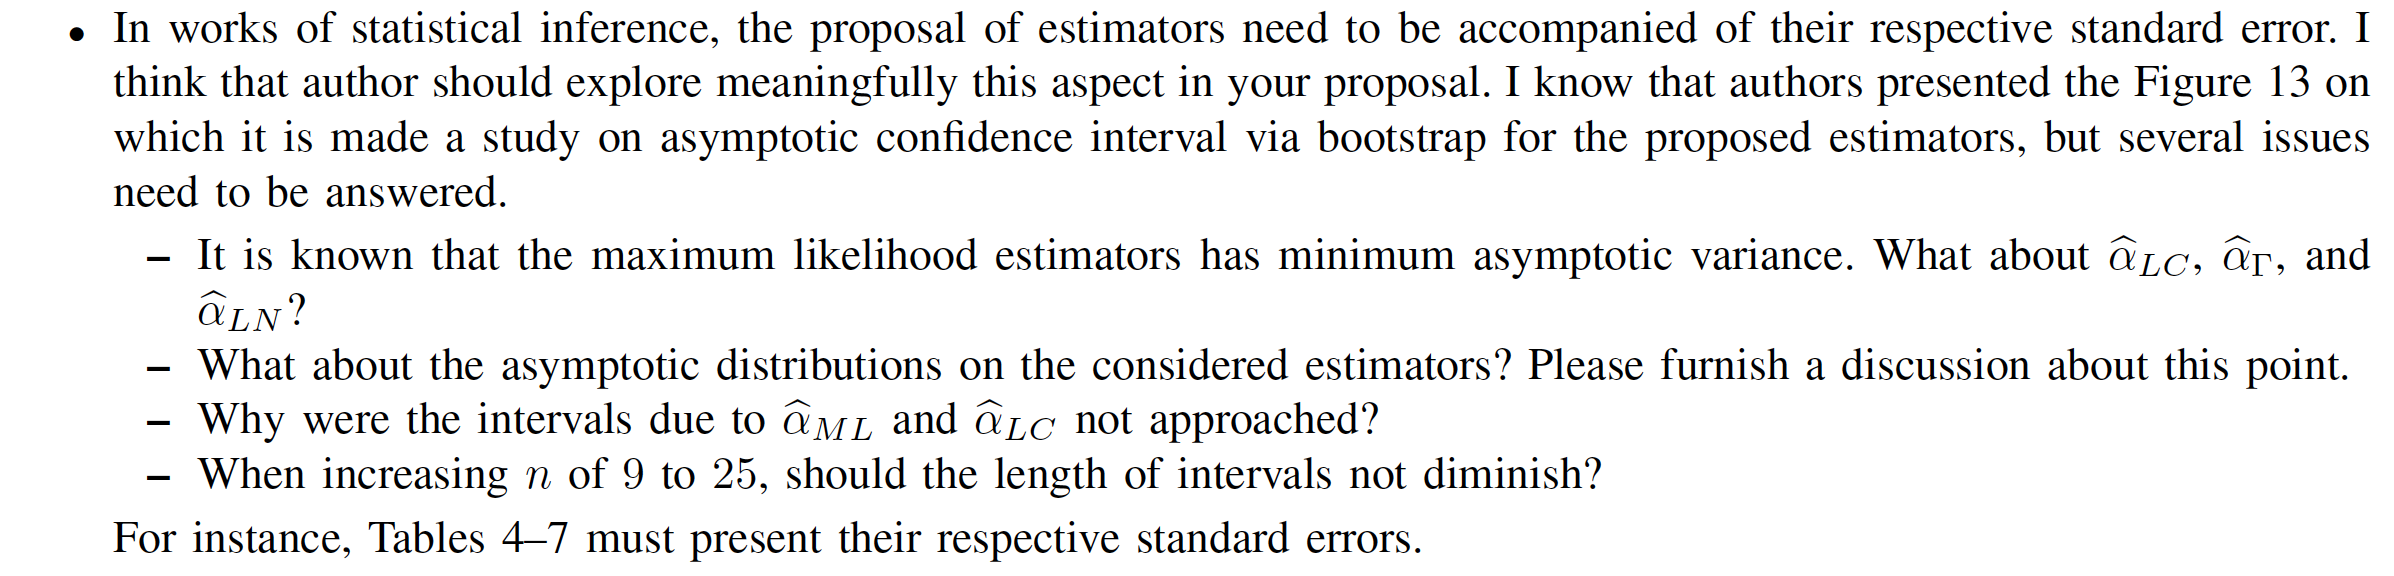
\includegraphics[width=\linewidth]{Critical}}
	
	\begin{enumerate}
		\item We added Table~5 with the sample variance of the estimators for several cases of $L$ and of $\alpha$, and its corresponding analysis.
		
		\item We performed new Monte Carlo experiments to assess the distribution of the proposed estimators.
		We included Figs.~5 and~6. 
		The former displays the estimators' sample density for $\alpha=-3$, $L=3$ and several sample sizes including $n=500$. 
		The latter exibits the sample density function for different values of the texture parameter for samples of size $500$. 
		We also present the values of skewness, kurtosis in Tables~4 and~5, respectively. We analyzed these figures and tables, and draw conclusions about the finite-sample and asymptotic distributions of the estimators.
		
		\item Thank you very much for this careful observation. There was an error in Fig.~15. We fixed this error and also added Table~9, which shows the length of the bootstrap confidence intervals.
		
		\item It can be seen in Table~9 that the length of the confidence intervals decrease as the sample size increases. It is important to note that, for $n=9$, neither ML or LC methods converge. 
		For this reason the confidence intervals for these cases are not shown. Tables~4 to~7 are now Tables~6 to~10. 
		All the new tables show the estimates accompanied by their respective confidence intervals as measures of the estimation error. 
	\end{enumerate}
	
	
	
	
	\subsection{Detailed comments}
	
	\fbox{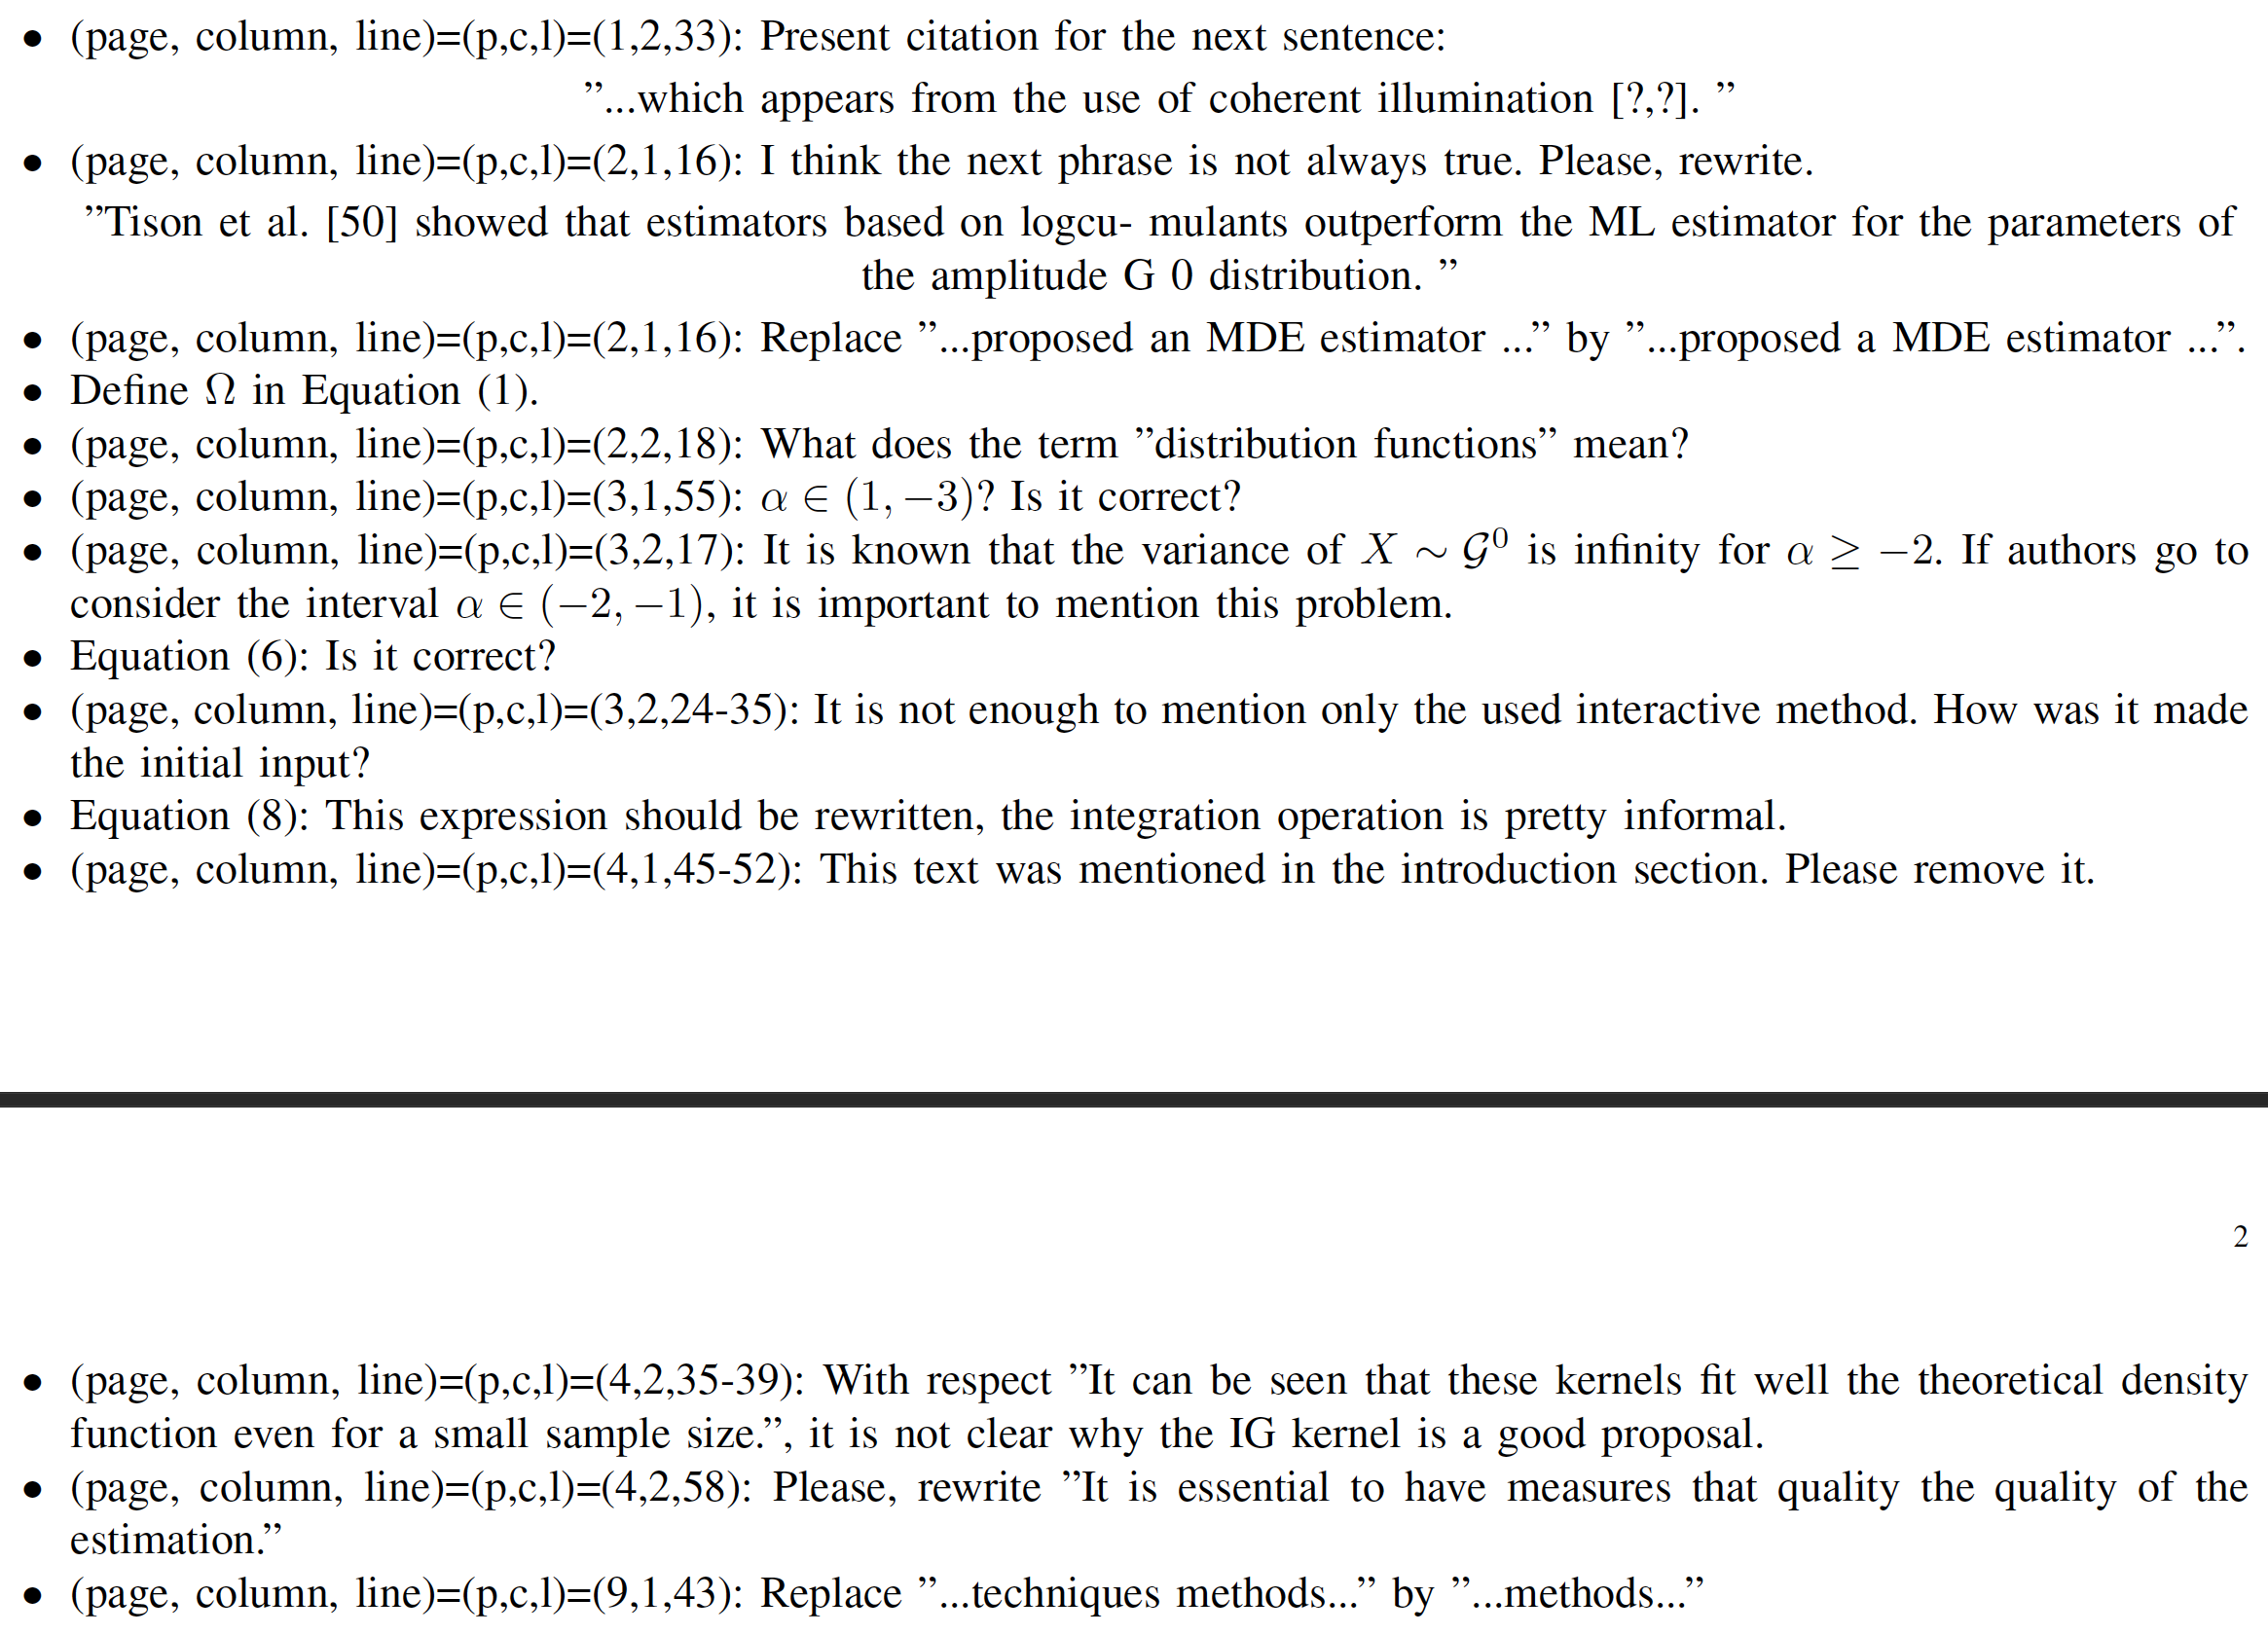
\includegraphics[width=\linewidth]{Detailed}}
	
	\AR We have made the following changes:
	\begin{itemize}
		\item We have added the reference by \citet{SARImageStatisticalModelingPartISinglePixelStatisticalModels}, which is a modern and comprehensive survey about speckle.
		\item Than you very much for this deep observation. We have rephrased our statement, and now we say that
		\begin{quote}
			Tison et al.~[50] showed that estimators based on logcumulants 
			are well-suited to model amplitude single-look data from urban areas, where very large values are frequently observed.
			Nevertheless, that work overlooks the fact that estimation under the $\mathcal G^0$ distribution is more sensitive to very small values rather than to extremely large ones.
			In this work, we explore this fact and propose suitable solutions using kernels.
		\end{quote}
		\item We struggled with this point, as English is not our native language, and we found the following answer in \url{https://forum.wordreference.com/threads/an-or-a-before-an-acronym-starting-with-m-h.2554395/}
		\begin{center}
			\includegraphics[width=\linewidth]{AorAN.png}
		\end{center}
		According this recommendation, we write ``an MDE''.
		\item We added ``where $\Omega$ is the parameter space.'' to the sentence after~(1).
		\item We changed the text as follows:
		\begin{quote}
			In particular, several measures have been proposed to reflect the closeness  \DIFdelbegin \DIFdel{between two distribution functions.} \DIFdelend \DIFaddbegin \DIFadd{among the models that describe samples.}\DIFaddend
		\end{quote}
		\item It was wrong; we corrected it and now it reads ``$\alpha \in (-3,-1)$''.
		\item We have justified our choice of texture parameters for the study, including a point in which the variance is infinite, with the following new paragraph:
		\begin{quote}
			Although the variance of a $\mathcal{G}^0$-distributed random variable is infinite when $\alpha>-2$, cf.~(3), we need to assess the behavior of estimators in such cases.
			As noted by, among others Ref.~[15, Fig.~5], one should expect that extremely heterogeneous samples as, for instance, those from urban areas, are described in this region of the parameter space.
		\end{quote}
		\item Equation~(6) is correct because we only consider the terms that depend on $\alpha$, which are those involved in the minimization.
		\item We added the following text to explain which was the initial point that was considered in the algorithm.
		\begin{quote}
			taking as a starting point $\alpha_0$ the alpha moment estimator when it exists. Otherwise we consider $\alpha_0=-1.5$.
		\end{quote}
		\item We rewrote equation~(8) as 
		\begin{equation}
			d_{\text{{T}}}(f_{\text{{V}}},f_{\text{{W}}})=\int_{S}\frac{\big(f_{\text{{V}}}(x)-f_{\text{{W}}}(x)\big)^2}{f_{\text{{V}}}(x)+f_{\text{{W}}}(x)}dx,
			\label{DT}
		\end{equation}
		
		\item Following your request this paragraph was deleted.
		\item We explain this in the text as follows:
		\begin{quote}
			It can be seen that these kernels fit reasonably well the theoretical density function even for a small sample size. The IG kernel presents a good approximation to the true density function at the center of the function although heavier tails are observed. The $\Gamma$ and LN kernels show a better fit, with the latter kernel having a higher kurtosis than the other kernels.
		\end{quote}
		\item We changed the text as follows:
		\begin{quote}		
			It is essential to have measures that \DIFdelbegin \DIFdel{quality} \DIFdelend \DIFaddbegin \DIFadd{quantify }\DIFaddend the quality of the estimation. 
		\end{quote}
		\item We deleted the word ``techniques''.
	\end{itemize}
	
	\bibliographystyle{agsm}
	\bibliography{Biblio}
	
\end{document}
